% Proposal Skripsi
% Muhammad Ghazali - 0606036
\documentclass[a4paper, 12pt, oneside]{report}
\usepackage{setspace}
\usepackage{graphicx, times}
\usepackage[bahasa]{babel}
\usepackage{listings}
\usepackage{tikz}
\usepackage{tabularx}
\usepackage{graphicx}
\usepackage{pifont}
\usepackage[top=3cm, bottom=3cm, left=4cm, right=3cm]{geometry}

\selectlanguage{bahasa}
%Gummi|063|=)
\title{\textbf{Membangun Web API dengan menggunakan JSON sebagai format serialisasi data}}
\author{
Muhammad Ghazali\\
Program Studi Teknik Informatika\\
Fakultas Teknik\\
Universitas Widyatama
\\\texttt{<muhammad.ghazali@widyatama.ac.id>}
}
\date{\today}

\begin{document}

\maketitle

\onehalfspacing
\tableofcontents
\setcounter{secnumdepth}{5}
\setcounter{tocdepth}{7}

\addcontentsline{toc}{chapter}{\listfigurename}
\listoffigures

\addcontentsline{toc}{chapter}{\listtablename}
\listoftables

% most research papers have an abstract, then there is a predefined commands
% for telling LaTeX which part of the content makes up the abstract. This
% should appear in its logical order, therefore, after the top matter, but
% before the main sections of the body.
\begin{abstract}
\onehalfspacing LayangLayang Mobile (LLM) merupakan salah perusahaan yang bergerak di bidang \textit{mobile application development}. Saat ini LayangLayang Mobile sedang mengembangkan sebuah produk bernama CampusLife. Produk yang dikembangkan tersebut merupakan aplikasi \textit{mobile} yang bertujuan untuk membantu civitas kampus mengakses informasi relevan tentang kampus mereka.

\onehalfspacing Setiap informasi yang ditampilkan melalui aplikasi \textit{mobile} CampusLife merupakan data yang sudah diolah dan diambil dari Web API\footnote{http://en.wikipedia.org/wiki/Web\_API} CampusLife. Saat ini LLM belum memiliki Web API tersebut. Berdasarkan kondisi tersebut, penulis bekerjasama dengan LLM untuk membangun Web API CampusLife. Web API yang akan dibangun bertujuan untuk membuka akses secara tidak langsung ke \textit{data store}\footnote{http://en.wikipedia.org/wiki/Data\_store} yang tersimpan di salah satu layanan \textit{Database as a Service}\footnote{http://en.wikipedia.org/wiki/Cloud\_database} yang digunakan oleh LLM di AppFog\footnote{http://www.appfog.com/}. Seluruh data-data \textit{event} yang tersimpan di \textit{data store} akan diolah oleh Web API menjadi data dengan format yang dapat dikonsumsi dengan mudah oleh aplikasi \textit{mobile} CampusLife. Proses pengelohan tersebut dinamakan serialisasi data\footnote{Lihat bagian Landasan teori: Serialiasi Data}.

\onehalfspacing Dalam penelitian ini penulis akan memilih format serialisasi data JSON untuk digunakan merepresentasikan setiap data-data \textit{event} dalam format yang dapat dikonsumsi oleh aplikasi \textit{mobile} CampusLife. Penulis memilih format serialisasi data JSON karena JSON lebih mudah dibaca ditulis dan dibaca oleh mesin (komputer) dan manusia. Selain itu JSON lebih mudah untuk diproses karena memiliki struktur yang lebih sederhana dibandingkan XML\cite{json-fat-free}\cite{json-vs-xml-debate}.

\begin{flushleft}
\onehalfspacing Kata kunci: Web API, JSON, Format Serialisasi Data
\end{flushleft}

\end{abstract}

% isi latar belakang dan masalah dibuat dengan mengikuti panduan:
% http://romisatriawahono.net/2012/06/18/kiat-menyusun-alur-latar-belakang-masalah-penelitian/
\chapter{Pendahuluan}
\section{Latar Belakang dan Masalah}
% menjelaskan obyek penelitian
\onehalfspacing CampusLife adalah \textit{mobile information directory application} yang dikembangkan oleh LayangLayang Mobile (LLM) untuk menyediakan informasi yang relevan kepada civitas kampus. Salah satu fitur utama yang akan dirilis dalam waktu dekat adalah menyediakan informasi \textit{event}-\textit{event} terbaru kepada civitas kampus. 

\onehalfspacing Setiap informasi yang ditampilkan melalui aplikasi \textit{mobile} CampusLife merupakan data yang sudah diolah dan diambil dari Web API\footnote{http://en.wikipedia.org/wiki/Web\_API} CampusLife. Saat ini LLM belum memiliki Web API dan penulis berniat untuk membangun Web API tersebut. Web API yang akan dibangun bertujuan untuk membuka akses secara tidak langsung ke \textit{data store}\footnote{http://en.wikipedia.org/wiki/Data\_store} yang tersimpan di salah satu layanan \textit{Database as a Service}\footnote{http://en.wikipedia.org/wiki/Cloud\_database} yang digunakan oleh LLM di AppFog\footnote{http://www.appfog.com/}. Seluruh data-data \textit{event} yang tersimpan di \textit{data store} akan diolah oleh Web API menjadi data dengan format yang dapat dikonsumsi dengan mudah oleh aplikasi \textit{mobile} CampusLife. Proses pengolahan tersebut dinamakan serialisasi data\footnote{Lihat bagian Landasan teori: Serialiasi Data}.

\onehalfspacing Dalam penelitian ini penulis akan memilih format serialisasi data JSON untuk digunakan merepresentasikan setiap data-data \textit{event} dalam format yang dapat dikonsumsi oleh aplikasi \textit{mobile} CampusLife. Penulis memilih format serialisasi data JSON karena JSON lebih mudah dibaca ditulis dan dibaca oleh mesin (komputer) dan manusia. Selain itu JSON lebih mudah untuk diproses karena memiliki struktur yang lebih sederhana dibandingkan XML\cite{json-fat-free}\cite{json-vs-xml-debate}.

% menjelaskan rangkuman penelitian
\onehalfspacing \textit{Smartphone} sebagai perangkat tempat aplikasi \textit{mobile} CampusLife berjalan, merupakan salah satu \textit{mobile computing devices} yang memiliki masa hidup baterai dan ketersediaan \textit{bandwidth} yang terbatas.\cite{challenging-issues-and-limitations-of-mobile-computing}. Dengan kedua keterbatasan tersebut, dalam penelitian ini penulis akan mengkaji penerapan format serialisasi data JSON yang efektif untuk menghasilkan ukuran data yang optimal saat pengiriman data berlangsung dari Web API ke aplikasi \textit{mobile} CampusLife. Hasil akhir yang diharapkan adalah format serialisasi data JSON mampu menghasilkan ukuran data yang optimal untuk dikonsumsi oleh aplikasi \textit{mobile}.

% Pada bagian ini jelaskan rumusan masalah yang akan diteliti
\section{Rumusan Masalah}
\onehalfspacing Berdasarkan latar belakang masalah yang telah dipaparkan, maka masalah yang akan diteliti dalam penelitian ini dapat dirumuskan sebagai berikut:
\begin{enumerate}
  \item Bagaimana membangun Web API dengan efektif agar data yang dikirimkan dapat memiliki ukuran data yang optimal untuk dikonsumsi oleh aplikasi \textit{mobile} CampusLife?
  \item Bagaimana JSON dapat diterapkan secara efektif agar data yang dihasilkan dapat memiliki ukuran data yang optimal untuk dikonsumsi oleh aplikasi \textit{mobile} CampusLife?
\end{enumerate}

% Tujuan dan manfaat penelitian
\section{Tujuan dan Manfaat Penelitian}
\onehalfspacing Tujuan dari pelaksanaan penelitian tugas akhir yang dilakukan penulis adalah:
\begin{enumerate}
  \item Membangun purwa-rupa Web API yang mampu mengirimkan data dengan ukuran data yang optimal untuk dikonsumsi oleh aplikasi \textit{mobile} CampusLife.
  \item Menerapkan JSON dengan efektif untuk menghasilkan data dengan ukuran data yang optimal untuk dikonsumsi oleh aplikasi \textit{mobile} CampusLife.
\end{enumerate}

\onehalfspacing Penulis mengharapkan hasil penelitian ini akan membawa manfaat positif bagi kepentingan dunia akademik dan praktis dalam hal penerapan format serialisasi data JSON untuk menghasilkan ukuran data yang optimal untuk dikonsumsi oleh aplikasi \textit{mobile}.

\section{Batasan Masalah}
\onehalfspacing Untuk memperjelas ruang lingkup pelaksanaan penelitian, penulis memiliki batasan masalah meliputi:
\onehalfspacing
\begin{enumerate}
  \item Pembangunan Web API hanya akan sampai pada tahap purwa-rupa.
  \item Pembangunan Web API hanya akan meliputi API untuk mengambil data-data \textit{event}.
  \item JSON hanya mampu merepresentasikan data dalam bentuk teks, oleh karena itu data yang akan digunakan hanya terbatas pada data yang berbasis teks.
  \item Skema data \textit{event} akan disediakan oleh pihak LLM.
  \item Dikarenakan keterbatasan waktu yang dimiliki oleh penulis, maka demo untuk mengakses Web API tidak jadi dilakukan melalui aplikasi \textit{mobile}.
  \item Penulis akan melakukan demo untuk mengakses Web API melalui Apache Benchmark\footnote{http://httpd.apache.org/docs/2.4/programs/ab.html} dalam lingkungan lokal yang terisolasi.
  \item Tidak membahas mengenai keamanan perangkat lunak, data dan jaringan.
  \item Pengembangan perangkat lunak menggunakan sebagian praktek dari \textit{Agile} dan tidak akan membahas \textit{Agile} secara komprehensif.
\end{enumerate}

\section{Metodologi Penelitian}
\onehalfspacing Adapun tahapan penelitian yang akan dilakukan oleh penulis tahap-tahap berikut:
\begin{enumerate}
  \item Identifikasi masalah. Pada tahap ini penulis merumuskan masalah yang akan diteliti.
  \item Perumusan hipotesis. Pada tahap ini penulis merumuskan jawaban sementara dari permasalahan yang diteliti.
  \item Pengujian hipotesis. Pada tahap ini penulis menguji penerapan JSON terhadap Web API yang sudah dibangun dan pembangunan perangkat lunak akan dilakukan dengan menggunakan metodologi pengembangkan perangkat lunak \textit{Agile}. 
  \item Kesimpulan. Pada tahap ini penulis menganalisa hasil pengujian hipotesis.
\end{enumerate}

\onehalfspacing Adapun cara untuk menunjang penelitian dilakukan dengan melakukan studi kepustakaan, yaitu pengumpulan data dari artikel-artikel, jurnal dan buku-buku yang berhubungan dengan topik pembahasan di penelitian.

% sistematika penulisan
\section{Sistematika Penulisan}
Sistematika pembahasan laporan ini terdiri dari enam bab, yaitu:
\begin{description}
  \item[Bab I Pendahuluan] Pada bagian ini berisikan pendahuluan laporan yang berisi latar belakang, rumusan masalah, tujuan dan manfaat penelitian, batasan masalah, metode penelitian dan sistematika penulisan laporan.
  \item[Bab II Landasan Teori] Pada bagian ini akan dibahas landasan teori yang berkaitan dan digunakan selama masa penelitian.
  \item[Bab III Analisis Sistem] Pada bagian ini akan dibahas hasil analisis terhadap masalah.
  \item[Bab IV Perancangan Sistem] Pada bagian ini akan dibahas hasil perancangan sistem.
  \item[Bab V Implementasi dan Pengujian Sistem] Pada bagian ini akan dibahas proses implementasi dan pengujian sistem berdasarkan kriteria pengujian yang sudah ditentukan.
  \item[Bab VI Penutup] Pada bagian ini berisikan kesimpulan dan saran yang didapatkan dari hasil penelitian.
\end{description}

\chapter{Landasan Teori}

\section{Web API}
\onehalfspacing
\subsection{Apa itu Web API}

\onehalfspacing \textit{Application programming interface} (API) adalah sebuah protokol yang dimaksudkan untuk digunakan sebagai antarmuka oleh komponen perangkat lunak untuk berkomunikasi satu sama lain. Ketika digunakan dalam konteks pengembangan \textit{web}, API biasanya didefinisikan sebagai satu set \textit{Hypertext Transfer Protocol} (HTTP) \textit{request message}, dan disertai dengan \textit{response message} dalam \textit{Extensible Markup Language} atau \textit{JavaScript Object Notation}.

\onehalfspacing Praktek penerbitan Web API telah memungkinkan masyarakat \textit{web} seperti \newline pengembang aplikasi berbasis \textit{web} untuk membuat arsitektur terbuka untuk berbagi konten dan data antara masyarakat dan aplikasi. Dengan cara ini, konten yang dibuat dalam satu tempat dapat dikirimkan secara dinamis dan diperbaharui di beberapa lokasi di \textit{web} \cite{api-wikipedia}.

\subsection{Kenapa Web API}
Ketika Anda menjalankan aplikasi \textit{web}, pada saat tertentu Anda ingin menyediakan Web API. Berikut adalah berapa alasan yang umum kenapa perlu menyediakan Web API \cite{apis-linux-journal}:

\begin{enumerate}
  \item Untuk memungkinkan pengguna Anda mengakses data mereka melalui aplikasi pihak ketiga. Pertimbangkan berapa banyak pihak ketiga Twitter klien yang ada\footnote{http://en.wikipedia.org/wiki/List\_of\_Twitter\_services\_and\_applications}, semua menggunakan API Twitter\footnote{https://dev.twitter.com/}, daripada mengakses langsung ke situs \textit{web}\footnote{https://twitter.com/}. Hal yang sama berlaku untuk Amazon\footnote{http://www.amazon.com/} dan eBay\footnote{http://www.ebay.com/}, antara lain, yang memungkinkan pengguna untuk mengakses data katalog mereka dan bahkan mengeksekusi penjualan, semua melalui API.
  \item Untuk memungkinkan pengembang aplikasi mobile untuk mengakses situs Anda dengan mengirim dan mengambil data menggunakan HTTP.
  \item Untuk memungkinkan aplikasi Anda sendiri untuk mengakses data sendiri melalui panggilan Ajax\footnote{https://developer.mozilla.org/en/docs/AJAX}. Bila Anda membuat panggilan JavaScript di latar belakang menggunakan Ajax, kemungkinan besar Anda akan ingin menggunakan panggilan API, menerima XML atau JSON, bukan HTML yang membutuhkan \textit{parsing} lebih lanjut.
\end{enumerate}

\subsection{RESTful Web API}

\onehalfspacing RESTful Web API adalah Web API yang diimplementasikan dengan menggunakan HTTP dan prinsip-prinsip REST\footnote{http://www.ics.uci.edu/~fielding/pubs/dissertation/top.htm}. \textit{Representational State Transfer} (REST) mendefinisikan seperangkat prinsip arsitektur dimana penulis dapat merancang layanan Web yang berfokus pada sistem \textit{resource}, termasuk bagaimana keadaan \textit{resource} dipanggil dan ditransfer melalui HTTP oleh berbagai macam klien yang ditulis dalam bahasa (pemrograman) yang berbeda. Berikut adalah diagram yang mengilustrasikan proses saat klien mengirimkan \textit{request} dan RESTful Web API mengirimkan \textit{response} kepada klien:

\onehalfspacing
\begin{figure}[htp]
\centering
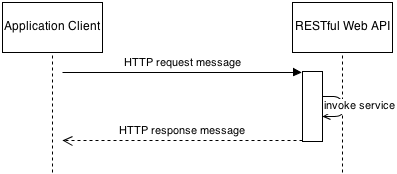
\includegraphics[scale=1.00]{images/RESTful-web-api.png}
\caption{RESTful Web API}
\label{RESTful Web API}
\end{figure}

\onehalfspacing Jika diukur dengan jumlah layanan Web yang menggunakannya, REST telah muncul dalam beberapa tahun terakhir sebagai model desain layanan Web yang dominan. Bahkan, REST memiliki dampak besar di dunia Web yang telah sebagian besar menggantikan desain antarmuka berbasis SOAP-WSDL dan karena REST memiliki gaya yang jauh lebih sederhana untuk digunakan \cite{ws-restful}. Berdasarkan informasi yang penulis dapatkan, pada saat laporan ini ditulis sudah lebih dari 5000 REST Web API yang diimplementasikan di dunia nyata\footnote{Web Services Directory http://www.programmableweb.com/apis/directory/1?protocol=REST}.

\section{Serialisasi data}

\onehalfspacing Dalam ilmu komputer, dalam konteks penyimpanan data dan transmisi, serialisasi (alias \textit{deflating}) adalah proses menerjemahkan struktur basis data atau kondisi objek ke dalam format yang dapat disimpan lebih lanjut dalam basis data (misalnya, dalam sebuah berkas atau \textit{buffer} memori, atau ditransmisikan melalui koneksi jaringan) dan dilakukan proses deserialisasi (alias \textit{inflating}) kembali di komputer lain \cite{serialization-wikipedia}. Proses serialisasi dan deserialisasi diilustrasikan dalam Gambar \ref{Proses Serialisasi}.

\onehalfspacing 
\begin{figure}[htp]
\centering
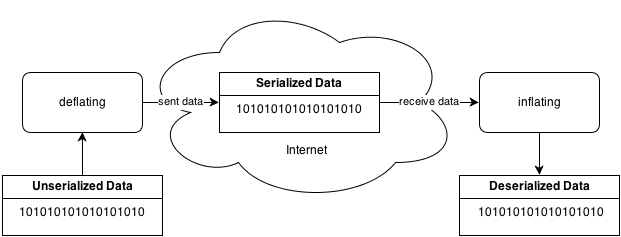
\includegraphics[scale=0.65]{images/serialization-process.png}
\caption{Proses Serialisasi}
\label{Proses Serialisasi}
\end{figure}

\onehalfspacing Pada saat penulis membuat laporan, sudah ada lebih dari 10 format serialisasi data\footnote{http://en.wikipedia.org/wiki/Comparison\_of\_data\_serialization\_formats}:
\begin{enumerate}
  \item ASN.1
  \item Bencode
  \item \textit{Candle Markup}
  \item \textit{Comma-separated values} (CSV)
  \item BSON
  \item \textit{D-Bus Message Protocol}
  \item JSON
  \item MessagePack
  \item Netstrings
  \item OGDL
  \item \textit{Property list}
  \item \textit{Protocol Buffers}
  \item S-expressions
  \item Sereal
  \item \textit{Structured Data eXchange Formats}
  \item Thrift
  \item \textit{eXternal Data Representation}
  \item XML
  \item XML-RPC
  \item YAML
\end{enumerate}

\section{JSON}

\subsection{Pengantar}
\onehalfspacing \textit{JavaScript Object Notation} (JSON) adalah format \textit{data interchange} ringan berbasis teks yang bersifat \textit{language-independent}\footnote{Dengan sifat seperti ini JSON bisa digunakan di banyak bahasa pemrograman, selama ada dukungan \textit{library} untuk bahasa pemrograman yang akan digunakan}. Relatif sangat mudah bagi manusia untuk membaca dan menulis JSON. Relatif sangat mudah pula bagi mesin (komputer) untuk mengurai dan menghasilkan JSON.

\onehalfspacing JSON dibuat dengan berbasiskan JavaScript, standar ECMA-262 Edisi 3 - Desember 1999\footnote{http://www.ecma-international.org/publications/standards/Ecma-262-arch.htm}. JSON merupakan format teks yang benar - benar bahasa independen tetapi menggunakan konvensi yang akrab bagi \textit{programmer} dari keluarga bahasa C, termasuk C, C + +, C\#, Java, JavaScript, Perl, Python, dan banyak lainnya. Properti ini membuat JSON sebagai bahasa \textit{data interchange} yang ideal\cite{introducing-json}.

\subsection{Struktur}
\onehalfspacing JSON dibangun di atas dua struktur:
\begin{enumerate}
  \item \textit{Collection of name/value pairs}. Dalam berbagai bahasa, struktur ini direalisasikan sebagai \textit{object}, \textit{record}, \textit{struct}, \textit{dictionary}, \textit{hash table}, \textit{keyed list}, atau \textit{associative array}.
  \item \textit{Ordered List}. Dalam kebanyakan bahasa, struktur ini direalisasikan sebagai \textit{array}, \textit{vector}, \textit{list}, atau \textit{sequence}.
\end{enumerate}

\onehalfspacing Kedua struktur tersebut adalah struktur data universal. Hampir semua bahasa pemrograman modern mendukung struktur tersebut dalam satu bentuk atau lain \cite{introducing-json}.

\subsection{Tipe Data yang Didukung JSON}
\onehalfspacing JSON dapat mewakili empat tipe primtif (\textit{string}, \textit{number}, \textit{boolean}, and \textit{null}) dan dua tipe terstruktur (\textit{object} and \textit{array}) \cite{rfc-4627}.

\onehalfspacing Sebuah \textit{object} adalah sebuah \textit{unordered collection} yang terdiri dari nol atau lebih pasangan nama/nilai, dimana sebuah nama adalah \textit{string} dan sebuah nilai adalah \textit{string}, \textit{number}, \textit{boolean}, \textit{null}, \textit{object}, atau \textit{array}.

\begin{figure}[htp]
\centering
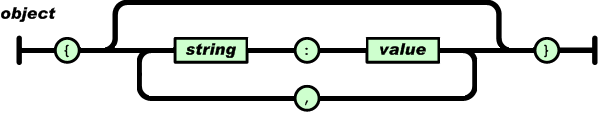
\includegraphics[scale=0.55]{images/object-json.png}
\caption{Diagram Sintaks untuk Tipe Object \cite{json-fat-free}}
\label{Diagram Sintaks untuk Tipe Object}
\end{figure}

\onehalfspacing \textit{Array} adalah rangkaian terurut yang terdiri dari nol atau lebih nilai.

\begin{figure}[htp]
\centering
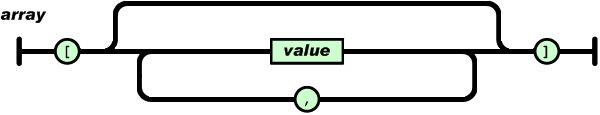
\includegraphics[scale=0.55]{images/array-json.png}
\caption{Diagram Sintaks untuk Tipe Array \cite{json-fat-free}}
\label{Diagram Sintaks untuk Tipe Array}
\end{figure}

\onehalfspacing \textit{Value} dapat berupa \textit{string} dalam tanda kutip ganda, \textit{number}, \textit{boolean}, \textit{object} atau \textit{array}. Struktur ini dapat diulang.

\onehalfspacing \textit{String} adalah rangkaian yang terdiri dari nol atau lebih karakter \textit{Unicode}\footnote{http://www.unicode.org/versions/Unicode6.2.0/}.

\begin{figure}[htp]
\centering
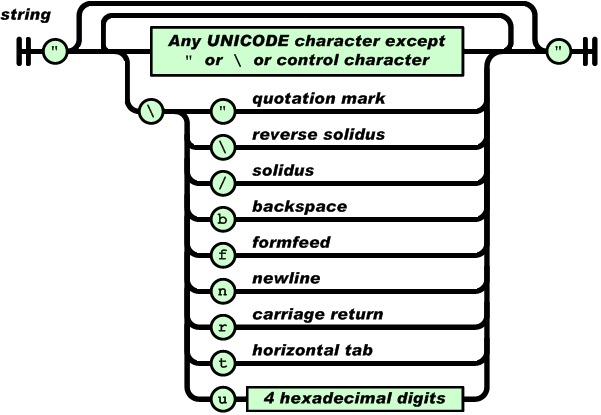
\includegraphics[scale=0.55]{images/string-json.png}
\caption{Diagram Sintaks untuk Tipe String \cite{json-fat-free}}
\label{Diagram Sintaks untuk Tipe String}
\end{figure}

\onehalfspacing \textit{Number} di JSON sama seperti tipe data \textit{number} di C atau Java, kecuali format oktal\footnote{Contoh angka dalam bentuk oktal 061 062 063} dan heksadesimal\footnote{Contoh angka dalam bentuk 9B0} tidak digunakan.

\begin{figure}[htp]
\centering
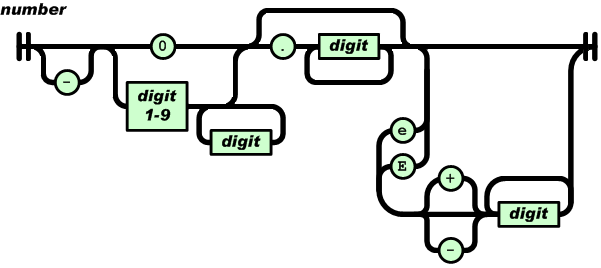
\includegraphics[scale=0.55]{images/number-json.png}
\caption{Diagram Sintaks untuk Tipe Number \cite{json-fat-free}}
\label{Diagram Sintaks untuk Tipe Number}
\end{figure}

\newpage
\subsection{Contoh-contoh}
\onehalfspacing Ini adalah contoh \textit{object} dalam format JSON:

\begin{lstlisting}[frame=single]
{
  "Image": {
    "Width": 800,
    "Height": 600,
    "Title": "View from 15th Floor",
    "Thumbnail": {
      "Url": "http://www.example.com/image/481989943",
      "Height": 125,
      "Width": "100"
    },
    "IDs": [116, 943, 234, 38793]
  }
}
\end{lstlisting}

\onehalfspacing Ini adalah contoh sebuah \textit{array} dalam format JSON yang berisi 2 \textit{object}:

\begin{lstlisting}[frame=single]
[
  {
    "precision": "zip",
    "Latitude": 37.7668,
    "Longitude": -122.3959,
    "Address": "",
    "City": "SAN FRANCISCO",
    "State": "CA",
    "Zip": "94107",
    "Country": "US"
  },
  {
    "precision": "zip",
    "Latitude": 37.371991,
    "Longitude": -122.026020,
    "Address": "",
    "City": "SUNNYVALE",
    "State": "CA",
    "Zip": "94085",
    "Country": "US"
  }
]
\end{lstlisting}

\section{XML}

\subsection{Pengantar}

\onehalfspacing \textit{Extensible Markup Language} (XML) adalah bahasa \textit{markup} yang mendefinisikan seperangkat aturan untuk \textit{document encoding} dalam format yang dapat terbaca oleh manusia dan mesin. Ini didefinisikan dalam spesifikasi XML 1.0\footnote{http://www.w3.org/TR/REC-xml/} yang dihasilkan oleh W3C.

\onehalfspacing Tujuan desain XML menekankan kesederhanaan, keumuman, dan kegunaan melalui Internet. XML adalah format data tekstual dengan dukungan kuat melalui Unicode. Meskipun desain XML berfokus pada dokumen, namun secara luas digunakan untuk menrepresentasikan struktur data yang berubah-ubah, misalnya dalam layanan web \cite{xml-wikipedia}.

\onehalfspacing Dikarenakan topik penelitian ini tidak membandingkan antara JSON versus XML dan tidak fokus ke XML, maka penulis hanya menjelaskan XML secara singkat.

\subsection{Contoh Dokumen XML}
\onehalfspacing Berikut adalah contoh dokumen XML dari tutorial W3Schools\footnote{http://www.w3schools.com/xml/cd\_catalog.xml}:

\begin{lstlisting}[frame=single]
<?xml version="1.0" encoding="ISO-8859-1"?>
<CATALOG>
	<CD>
		<TITLE>Empire Burlesque</TITLE>
		<ARTIST>Bob Dylan</ARTIST>
		<COUNTRY>USA</COUNTRY>
		<COMPANY>Columbia</COMPANY>
		<PRICE>10.90</PRICE>
		<YEAR>1985</YEAR>
	</CD>
	<CD>
		<TITLE>Hide your heart</TITLE>
		<ARTIST>Bonnie Tyler</ARTIST>
		<COUNTRY>UK</COUNTRY>
		<COMPANY>CBS Records</COMPANY>
		<PRICE>9.90</PRICE>
		<YEAR>1988</YEAR>
	</CD>
</CATALOG>
\end{lstlisting}

\subsection{Kritik Terhadap XML}

\onehalfspacing XML telah sering dikritik karena bertele-tele dan kerumitan yang dimiliki. Pemetaan model pohon dasar XML untuk tipe sistem bahasa pemrograman atau basis data bisa menjadi sulit, terutama ketika XML digunakan untuk pertukaran data yang sangat terstruktur antara aplikasi, yang dimana bukan tujuan desain utama XML \cite{xml-wikipedia}.

\onehalfspacing Walaupun XML bisa digunakan untuk \textit{data interchange}, namun, XML tidak cocok untuk \textit{data interchange}. Ini membawa banyak bagasi (baca: pengeluaran tambahan), dan tidak cocok dengan model data dari kebanyakan bahasa pemrograman. Ketika kebanyakan \textit{programmer} melihat XML untuk pertama kalinya, mereka terkejut melihat betapa jelek dan tidak efisiennya XML \cite{json-fat-free}.

\section{Menggunakan JSON daripada XML}

\onehalfspacing Pada dasarnya setiap hal selalu memiliki kelebihannya dan kekurangannya serta \textit{use case} masing-masing. Seperti yang sudah dijelaskan sebelumnya tentang kritik terhadap XML, pada bagian ini dijelaskan beberapa poin kenapa lebih memilih untuk menggunakan JSON daripada XML. Berikut adalah beberapa alasan tersebut:

\begin{enumerate}
  \item JSON lebih sederhana
  \begin{enumerate}
    \item JSON lebih sederhana dibandingkan XML. JSON memiliki tata bahasa yang jauh lebih kecil dan lebih mudah dipetakan langsung ke struktur data yang digunakan dalam bahasa pemrograman modern.
    \item JSON jauh lebih mudah bagi manusia untuk dibaca daripada XML. JSON juga lebih mudah untuk ditulis dan dibaca oleh mesin.
  \end{enumerate}
  \item JSON dapat dipetakan dengan lebih mudah untuk sistem berorientasi objek.
  \item JSON sudah diadopsi secara luas oleh banyak pihak di industri perangkat lunak \cite{json-continue-to-winning}\cite{json-continue-to-push}.
\end{enumerate}

\section{Agile Software Development}
\subsection{Pengantar}
\onehalfspacing Pengembangan perangkat lunak \textit{Agile} adalah sekelompok metode pengembangan perangkat lunak berdasarkan metode pengembangan \textit{iterative and incremental}\footnote{http://en.wikipedia.org/wiki/Iterative\_and\_incremental\_development}, di mana persyaratan dan solusi berkembang melalui kolaborasi. Ini mempromosikan perencanaan adaptif, perkembangan dan pengiriman yang evolusioner, pendekatan \textit{time-boxed}\footnote{http://en.wikipedia.org/wiki/Timeboxing} berulang, dan mendorong respon cepat dan fleksibel terhadap perubahan \cite{agile-wikipedia}.

\subsection{Manifesto Pengembangan Perangkat Lunak Agile}

\onehalfspacing Pada Februari 2001, 17 pengembang perangkat lunak\footnote{Kent Beck, Mike Beedle, Arie van Bennekum, Alistair Cockburn, Ward Cunningham, Martin Fowler, James Grenning, Jim Highsmith, Andrew Hunt, Ron Jeffries, Jon Kern, Brian Marick, Robert C. Martin, Stephen J. Mellor, Ken Schwaber, Jeff Sutherland, and Dave Thomas} bertemu di Snowbird, Utah, untuk membahas metode pengembangan ringan. Mereka menerbitkan manifesto untuk \textit{Agile Software Development} untuk menentukan pendekatan yang sekarang dikenal sebagai pengembangan perangkat lunak \textit{Agile} \cite{agile-wikipedia}.

\onehalfspacing Melalui manifesto tersebut mereka menghargai \cite{agile-manifesto}:
\begin{enumerate}
  \item Individu dan interaksi lebih dari proses dan sarana perangkat lunak
  \item Perangkat lunak yang bekerja lebih dari dokumentasi yang menyeluruh
  \item Kolaborasi dengan klien lebih dari negosiasi kontrak
  \item Tanggap terhadap perubahan lebih dari mengikuti rencana
\end{enumerate}

\onehalfspacing Demikian, walaupun mereka menghargai hal di sisi kanan, mereka lebih menghargai hal di sisi kiri. Arti dari item manifesto di sebelah kiri dalam konteks pembangunan perangkat lunak \textit{Agile} dijelaskan di bawah ini:

\begin{enumerate}
  \item Individu dan interaksi. Dalam pengembangan perangkat lunak \textit{Agile}, mengorganisir diri dan motivasi merupakan hal yang penting, seperti interaksi seperti \textit{co-location}\footnote{http://en.wikipedia.org/wiki/Colocation\_(business)} dan \textit{pair programming}\footnote{http://en.wikipedia.org/wiki/Pair\_programming}.
  \item Perangkat lunak yang bekerja (berfungsi dengan baik). Perangkat lunak yang bekerja akan lebih bermanfaat dan diterima daripada sekedar menyajikan dokumen untuk klien dalam pertemuan.
  \item Kolaborasi dengan klien. Daftar kebutuhan perangkat lunak tidak dapat \newline dikumpulkan secara menyeluruh pada awal siklus pengembangan perangkat lunak, sehingga keterlibatan terus menerus pelanggan atau pemangku kepentingan sangat penting.
  \item Tanggap terhadap perubahan. Pengembangan perangkat lunak \textit{Agile} difokuskan pada respon cepat terhadap perubahan dan pembangunan berkelanjutan.
\end{enumerate}

\subsection{Prinsip-prinsip di balik Manifesto Agile}
Manifesto pengembangan perangkat lunak \textit{Agile} didasarkan pada dua belas prinsip:
\begin{enumerate}
  \item Prioritas utama kami adalah memuaskan klien dengan menghasilkan perangkat lunak yang bernilai secara dini dan rutin.
  \item Menyambut perubahan kebutuhan, walaupun terlambat dalam pengembangan perangkat lunak. Proses \textit{Agile} memanfaatkan perubahan untuk keuntungan kompetitif klien.
  \item Menghasilkan perangkat lunak yang bekerja secara rutin, dari jangka waktu beberapa minggu sampai beberapa bulan, dengan preferensi kepada jangka waktu yang lebih pendek.
  \item Rekan bisnis dan pengembang perangkat lunak harus bekerja-sama tiap hari sepanjang proyek.
  \item Kembangkan proyek di sekitar individual yang termotivasi. Berikan mereka lingkungan dan dukungan yang mereka butuhkan, dan percayai mereka untuk menyelesaikan pekerjaan dengan baik.
  \item Metode yang paling efisien dan efektif untuk menyampaikan informasi dari dan dalam tim pengembangan perangkat lunak adalah dengan komunikasi secara langsung.
  \item Perangkat lunak yang bekerja adalah ukuran utama kemajuan.
  \item Proses \textit{Agile} menggalakkan pengembangan berkelanjutan. Sponsor-sponsor, pengembang-pengembang, dan pengguna-pengguna akan dapat mempertahankan kecepatan tetap secara berkelanjutan.
  \item Perhatian yang berkesinambungan terhadap keunggulan teknis dan rancangan yang baik meningkatkan \textit{Agility}.
  \item Kesederhanaan--seni memaksimalkan jumlah pekerjaan yang belum dilakukan--adalah hal yang amat penting.
  \item Arsitektur, kebutuhan, dan rancangan perangkat lunak terbaik muncul dari tim yang yang dapat mengorganisir diri sendiri.
  \item Secara berkala, tim pengembang berefleksi tentang bagaimana untuk menjadi lebih efektif, kemudian menyesuaikan dan menyelaraskan kebiasaan bekerja mereka.
\end{enumerate}

\subsection{Bagaimana Agile Berbeda}
\onehalfspacing Sebenarnya, satu bab laporan ini tidak akan cukup untuk membahas bagaimana \textit{Agile} berbeda dengan metodologi pengembangan perangkat lunak lainnya dikarenakan cakupan bahasannya yang luas, tetapi ada beberapa hal umum yang perlu diketahui tentang proyek-proyek pengembangan perangkat lunak yang menggunakan \textit{Agile}.

\onehalfspacing Pertama, peran-peran yang diterapkan di proyek-proyek \textit{Agile} lebih fleksibel. Ketika diterapkan dengan tepat, bergabung dengan tim \textit{Agile} seperti di dalam sebuah \textit{mini-startup} (alias \textit{startup company}). Orang-orang di dalam tim bekerja dengan penuh semangat dan mengerjakan apa yang bisa dilakukan untuk membuat proyek menjadi sukses tanpa memperhatikan jabatan atau peran yang diemban.

\newpage
\onehalfspacing Kedua, yang membuat \textit{Agile} berbeda dengan yang lain adalah proses analisis, desain, \textit{coding}, dan pengujian merupakan aktivitas yang kontinu. Itu berarti kegiatan ini tidak bisa berlangsung dalam sifat yang terisolasi lagi. Ilustrasi aktivitas yang kontinu tersebut bisa dilihat pada Gambar \ref{agile-process}.

\begin{figure}[htp]
\centering
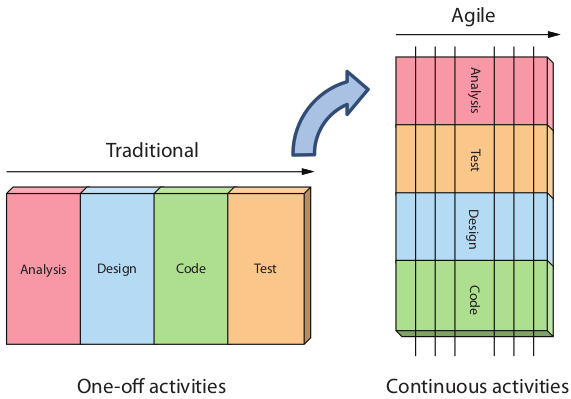
\includegraphics[scale=0.60]{images/agile-process.png}
\caption{Ilustrasi aktivitas kontinu di \textit{Agile} \cite{agile-samurai}}
\label{agile-process}
\end{figure}

\subsection{Beberapa Praktek Agile yang Diterapkan}

\onehalfspacing Mengingat pengetahuan penulis tentang Agile masih jauh dari cukup, cakupan pengerjaan dari purwa-rupa cukup kecil dan tim pengerjaan teknis yang hanya terdiri dari satu orang, yaitu penulis sendiri. Maka hanya sebagian kecil praktek \textit{Agile} yang diterapkan oleh penulis, yaitu:

\begin{enumerate}
  \item Mencatat daftar fitur dalam bentuk \textit{user story}
  \item Menerapkan jangka waktu 1 minggu untuk setiap iterasi
  \item Melakukan \textit{sprint planning} untuk merencanakan daftar tugas yang perlu dikerjakan selama iterasi berlangsung
\end{enumerate}

\chapter{Analisis Sistem}
\section{Roadmap Pengerjaan Purwa-rupa Web API}
\onehalfspacing Sebelum penulis memulai \textit{software development life cycle}, penulis terlebih dahulu menentukkan \textit{roadmap} dari pengembangan Web API yang terdiri dari 3 \textit{milestone} yang harus dipenuhi. Berikut daftar \textit{milestone} tersebut:
\begin{enumerate}
  \item M 1: \textit{Application Skeleton}. Pada \textit{milestone} ini penulis mempersiapkan struktur aplikasi\footnote{http://en.wikipedia.org/wiki/Skeleton\_(computer\_programming)}
  \item M 2: \textit{Make it works and right}. Pada \textit{milestone} ini penulis mengimplementasikan Web API sesuai dengan kebutuhan dan rancangan yang sudah ditentukan.
  \begin{enumerate}
    \item API untuk merespon permintaan konten event dalam format JSON
    \item API untuk merespon permintaan konten event dalam format XML
  \end{enumerate}
  \item M 3: \textit{Measuring}
    \begin{enumerate}
      \item Mengukur jumlah permintaan yang berhasil dilakukan dalam 90 detik ketika meminta konten event dalam format XML
      \item Mengukur jumlah permintaan yang berhasil dilakukan dalam 90 detik ketika meminta konten event dalam format JSON
      \item Membuktikan bahwa data yang dihasilkan dalam format JSON lebih kecil ukurannya dibandingkan data yang dihasilkan dalam format XMl
    \end{enumerate}
\end{enumerate}

\section{High-level Architecture CampusLife}
\onehalfspacing Secara umum CampusLife dibangun dengan menggunakan \textit{three-tier architecture} yang terdiri dari 3 tingkat, yaitu \textit{presentation}, \textit{logic} dan \textit{data}. CampusLife dibangun dengan menggunakan \textit{three-tier architecture} dengan tujuan agar pengembang aplikasi bisa melakukan perubahan dengan relatif mudah. Gambaran visual dari arsitektur CampusLife dapat dilihat pada gambar \ref{high-level-architecture-cl}:

\begin{figure}[htp]
\centering
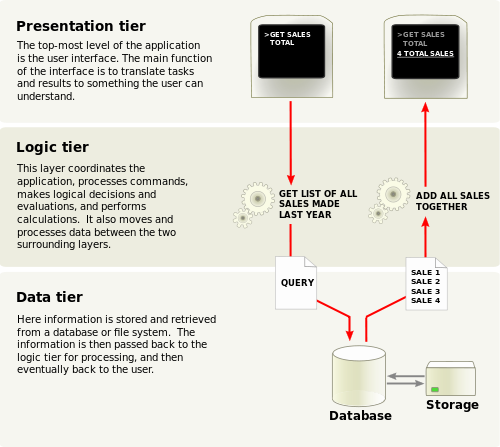
\includegraphics[scale=0.40]{images/test.png}
\caption{High-level architecture CampusLife}
\label{high-level-architecture-cl}
\end{figure}

\subsection{Presentation Tier}
\onehalfspacing \textit{Presentation tier} adalah \textit{tier} paling atas dari aplikasi CampusLife. \textit{Tier} ini menampilkan informasi terkait dengan layanan seperti menampilkan daftar event dan menampilkan daftar pengunjung event kepada pengguna melalui \textit{mobile application}. Layanan informasi seperti ini akan disediakan melalui Web API yang berada di \textit{logic tier} dan dapat diakses melalui \textit{client} seperti \textit{mobile application} dan \textit{browser}. Secara sederhana \textit{presentation tier} adalah tingkat dimana pengguna dapat mengakses aplikasi secara langsung. Dalam konteks pengerjaan penelitian tugas akhir ini, \textit{mobile application} CampusLife akan berada di \textit{tier} ini \cite{multitier-architecture-wikipedia}.

\subsection{Logic Tier}
\onehalfspacing \textit{Logic tier} adalah \textit{tier} yang berfungsi untuk mengontrol fungsionalitas aplikasi dengan melakukan pengolahan rinci. Contoh pengolahan rinci yang bisa dilakukan di \textit{tier} ini adalah mengambil daftar event. Dalam konteks pengerjaan penelitian tugas akhir ini, Web API akan berada di \textit{tier} ini \cite{multitier-architecture-wikipedia}.

\subsection{Data Tier}
\onehalfspacing \textit{Data tier} adalah \textit{tier} yang terdiri dari satu atau lebih \textit{server} basis data. Disini setiap informasi disimpan dan diambil. \textit{Tier} ini akan menjaga data tetap netral dan indenpenden dari \textit{application server} atau \textit{business logic}. Selain itu dengan memberikan data di \textit{tier} sendiri akan meningkatkan \textit{scalability} dan \textit{performance}. Dalam konteks pengerjaan penelitian tugas akhir ini, penulis menggunakan MongoDB\footnote{http://www.mongodb.org/} sebagai basis data di \textit{tier} ini \cite{multitier-architecture-wikipedia}.

\subsection{Keuntungan dari Arsitektur Three-tier}
\onehalfspacing CampusLife dibangun dengan menggunakan arsitektur \textit{three-tier} untuk mendapatkan beberapa keuntungan berikut:

\begin{enumerate}
  \item Lebih mudah untuk memodifikasi atau mengganti \textit{tier} apapun tanpa mempengaruhi \textit{tier} lainnya.
  \item Memisahkan aplikasi dan fungsi \textit{database} berarti \textit{load balancing} yang lebih baik.
\end{enumerate}

\subsection{Ruang Lingkup Pengerjaan}
\onehalfspacing Berdasarkan batasan masalah yang sudah penulis jelaskan di Bab 1, berikut adalah ruang lingkup pengerjaan yang penulis perlu dilakukan untuk membangun Web API:
\begin{enumerate}
  \item Membangun Web API
  \item Implementasi rancangan skema basis data di MongoDB
\end{enumerate}

\subsection{Daftar Kebutuhan yang harus dipenuhi}
\onehalfspacing Sebelum Web API dibangun, penulis menentukan terlebih dahulu daftar kebutuhan fungsional yang ada di Web API. Berikut daftar kebutuhan fungsional dan non-fungsional yang harus ada di Web API:
\begin{enumerate}
    \item Web API harus mampu untuk merespon permintaan daftar event dalam format JSON
    \item Web API harus mampu untuk merespon permintaan daftar event dalam format XML
    \item Web API harus mampu untuk merespon permintaan konten detail event dalam format JSON
    \item Web API harus mampu untuk merespon permintaan konten detail event dalam format XML
    \item Data yang dihasilkan Web API harus memiliki ukuran yang optimal sehingga aplikasi mobile dapat mengambil data dengan waktu yang relatif singkat
\end{enumerate}

\onehalfspacing Dari kelima daftar kebutuhan di atas, daftar kebutuhan ke-5 merupakan kebutuhan non-fungsional dan sisanya merupakan daftar kebutuhan fungsional.

Mengingat penulis mempraktekkan \textit{Agile} untuk membangun Web API ini, maka perlu diketahui dalam sehari-harinya setiap daftar kebutuhan fungsional dan non-fungsional tersebut biasa disebut dengan \textit{User Story}\footnote{Lebih detail tentang \textit{user story} silahkan baca di Bab 2 Landasan Teori} dan semua daftar \textit{user story} tersebut ditempatkan ke dalam \textit{Product Backlog}.

\subsection{Pola Alur Kerja Ketika Mengumpulkan Daftar Kebutuhan}

\onehalfspacing Ketika melakukan pengumpulan daftar kebutuhan penulis menemukan pola alur kerja sebagai berikut:

\begin{enumerate}
  \item Membuat \textit{user story} format singkat
  \item Membuat \textit{user story} format lengkap
\end{enumerate}

\newpage

\subsubsection{Membuat User Story format singkat}

\onehalfspacing Pada prakteknya jika penulis sedang dalam keadaan yang terburu-buru, penulis biasanya mencatat fitur-fitur baru yang akan dikembangkan dengan format singkat. Berikut adalah contoh daftar fitur yang dibuat dengan \textit{user story} format singkat:

\begin{enumerate}
  \item \textit{List upcoming events}
  \item \textit{Display upcoming competitions}
  \item \textit{Display event details}
\end{enumerate}

\onehalfspacing Poin penting yang perlu diingat ketika membuat \textit{user story} format singkat adalah:

\begin{enumerate}
  \item Mencatat \textbf{apa yang harus dilakukan oleh perangkat lunak}
  \item Mendeskripsikan fitur dengan \textbf{sesingkat dan sejelas mungkin}
\end{enumerate}

\onehalfspacing Tidak ada yang tahu hari esok seperti apa, \textbf{jangan tergoda untuk mendeskripsikan sedetail mungkin} ketika membuat \textit{user story} format singkat.

\subsubsection{Membuat User Story format panjang}

\onehalfspacing Pada prakteknya, penulis membuat \textit{user story} format panjang setelah mendefinisikan fitur dalam \textit{user story} format panjang. Berikut adalah format \textit{user story} format panjang:

\begin{lstlisting}[frame=single]
As a <type of user>
I want <some goal>
so that <some reason>
\end{lstlisting}

Berikut adalah format panjang yang diberi anotasi:

\begin{lstlisting}[frame=single]
As a <type of user> => Who is this story for
I want <some goal> => What they want to do
so that <some reason> => Why they want to do it
\end{lstlisting}

\onehalfspacing Setelah \textit{user story} format panjang dibuat, biasanya penulis meneruskan dengan menentukan \textit{acceptance criteria} untuk masing-masing \textit{user story} tersebut. \textit{Acceptance criteria} tersebut akan digunakan saat melakukan \textit{acceptance testing}.

\subsection{Acceptance Criteria}

\onehalfspacing \textit{Acceptance criteria} merupakan salah \textit{requirements artifact} yang akan berguna saat \textit{acceptance testing} untuk menentukan apakah kebutuhan sudah terpenuhi atau belum \cite{acceptance-testing-wikipedia}. Berikut adalah daftar masing-masing \textit{acceptance criteria} untuk setiap masing-masing \textit{user story}:
\begin{enumerate}
  \item \textit{Get Event Details Acceptance Criteria}
    \begin{enumerate}
      \item \textit{Scenario 1: Event Details request should return response in JSON}
      \item \textit{Scenario 2: Event Details request should return response in XML}
      \item \textit{Scenario 3: Unsupported Content-Type should return HTTP 406 code}
    \end{enumerate}
  \item \textit{Get Event List Acceptance Criteria}
    \begin{enumerate}
      \item \textit{Scenario 1: Event List request should return response in JSON}
      \item \textit{Scenario 2: Event List request should return response in XML}
      \item \textit{Scenario 3: Unsupported Content-Type should return HTTP 406 code}
    \end{enumerate}
\end{enumerate}

\onehalfspacing Setiap masing-masing skenario dari \textit{acceptance criteria} di atas diekspresikan dalam format \textit{Given When Then} \cite{introducing-bdd}\cite{whats-in-story}. Detail masing-masing dari setiap \textit{acceptance criteria} diatas bisa dilihat pada lampiran \ref{lampiran:a}.

\chapter{Perancangan Sistem}

\onehalfspacing Sebelum membaca lebih lanjut bab ini, para pembaca perlu mengetahui bahwa saat melakukan pemodelan, penulis mempraktekkan \textit{Just Barely Good Enough modelling}\cite{jbge-scott}. Jadi, jangan terkejut jika Anda menemukan model yang diperlihatkan di bab ini mungkin tidak "benar" menurut perspektif Anda karena saat itu model yang dibuat dianggap cukup berdasarkan pemahaman dan situasi yang dihadapi oleh penulis pada saat proses pemodelan berlangsung.

\section{Arsitektur Teknis Web API}

Untuk merancang arsitektur teknis dari Web API, penulis menggunakan \textit{free-form diagram}. Model arsitektur teknis yang dibuat digambarkan pada papan tulis dan model tersebut dapat dilihat pada gambar \ref{arsitektur-teknis-web-api}

\newpage

\begin{figure}[htp]
\centering
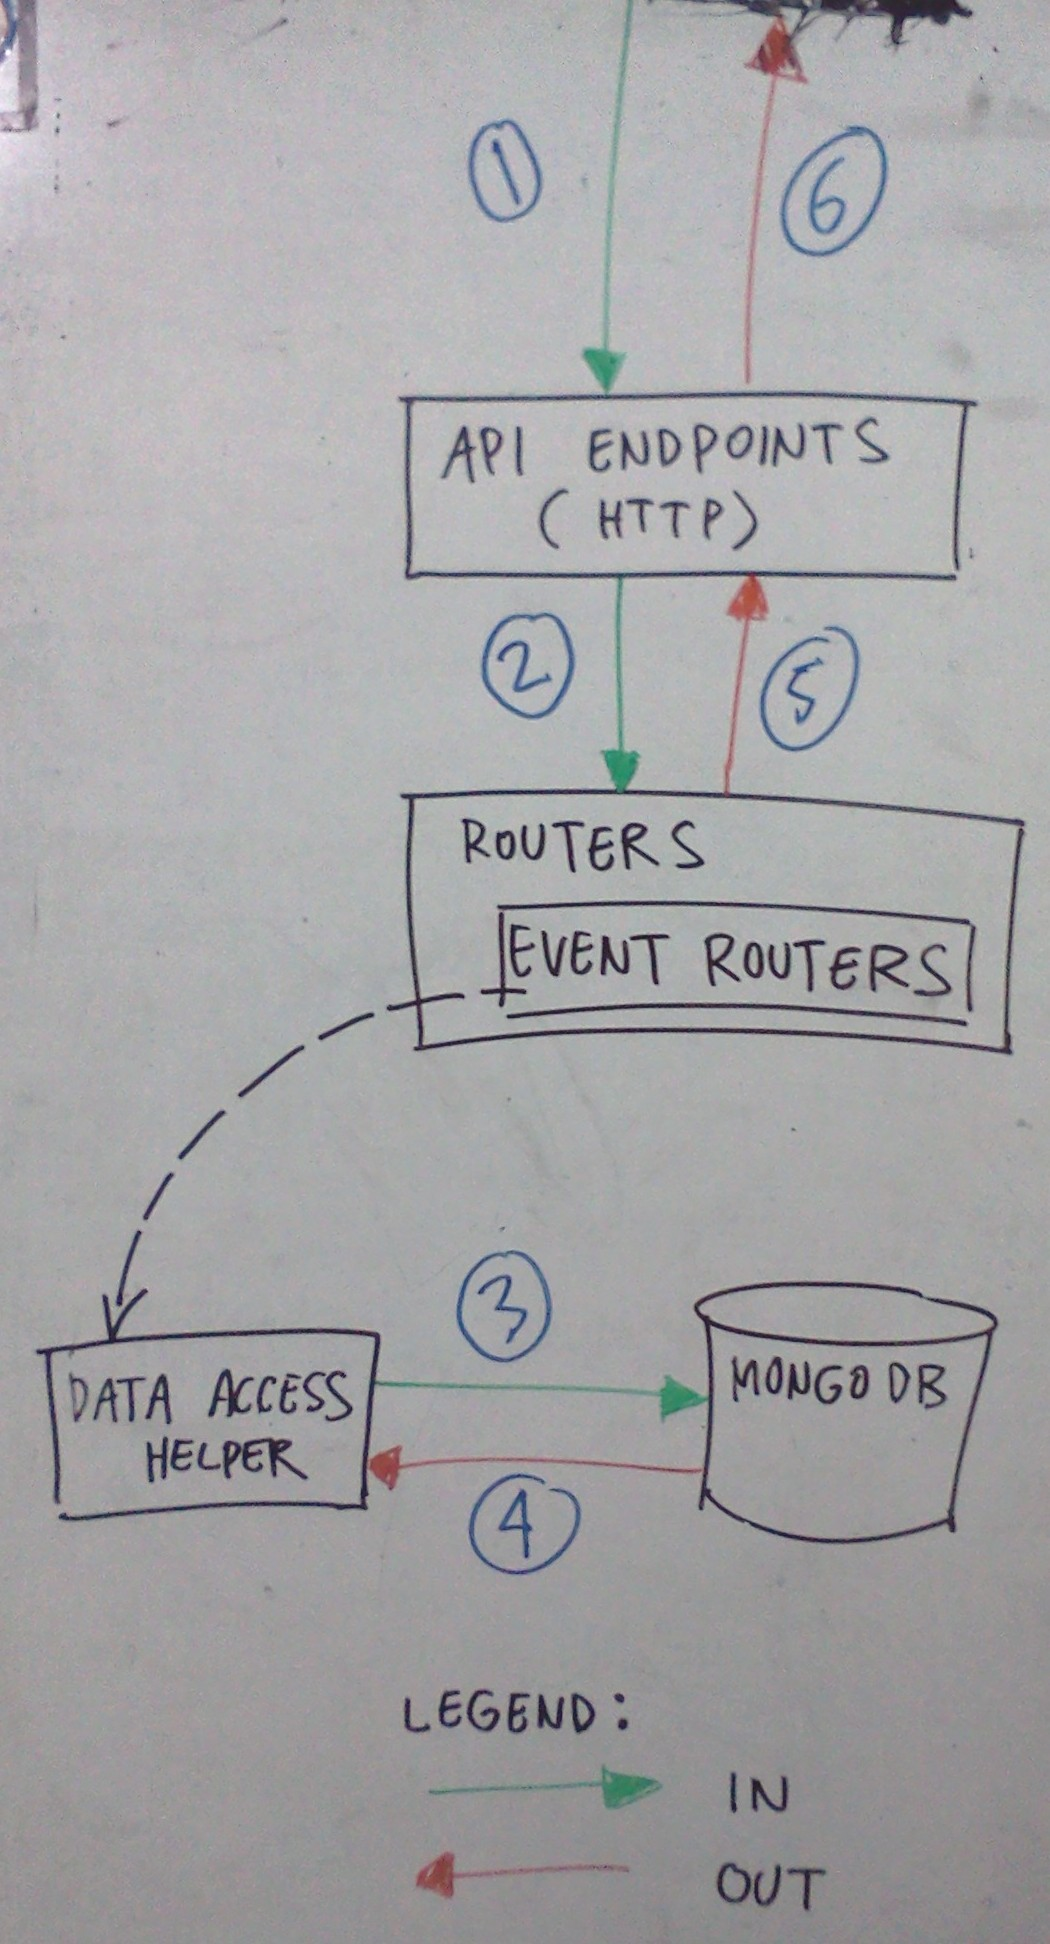
\includegraphics[scale=0.20]{images/arsitektur-teknis-web-api.jpg}
\caption{Model Arsitektur Teknis Web API dalam Free-form Diagram}
\label{arsitektur-teknis-web-api}
\end{figure}

\onehalfspacing Dikarenakan penulis menggunakan \textit{free-form diagram} untuk merancang arsitektur teknis dari Web API, berikut adalah keterangan dari beberapa bagian dari model di atas:

\begin{enumerate}
  \item \textit{HTTP Request} masuk dari \textit{client} melalui salah satu \textit{API endpoint}.
  \item \textit{HTTP Request} yang masuk akan diproses lebih lanjut oleh \textit{Routers}
  \item \textit{Routers} akan memiliki \textit{Data Access helper} untuk mengakses data mentah di MongoDB
  \item \textit{Routers} mendapatkan data untuk kemudian diolah sesuai dengan format yang diminta oleh \textit{client}
  \item \textit{HTTP Response} dikirimkan kepada \textit{client}
\end{enumerate}

\section{Service Interaction Model}

\onehalfspacing Pada bagian ini akan berisi laporan mengenai hasil pemodelan yang penulis lakukan saat melakukan perancangan sistem. Untuk mendapatkan gambaran dengan jelas mengenai sistem yang akan dibangun, penulis melakukan pemodelan interaksi antara \textit{client} dan Web API \textit{server}. Model tersebut dibuat dalam bentuk \textit{UML Sequence Diagram} dan digambarkan pada papan tulis. Namun, dalam laporan ini penulis memperlihatkan hasil pemodelan yang sudah dirubah ke dalam bentuk digital.

\onehalfspacing Saya asumsikan para pembaca sudah mengetahui penggunaan dasar dari \textit{UML Sequence Diagram}, jika belum mohon untuk memahami terlebih dahulu penggunaan dasar \textit{UML Sequence Diagram}\footnote{http://www.agilemodeling.com/artifacts/sequenceDiagram.htm}.

\newpage

\subsection{Permintaan Detail Event dalam format JSON}

\onehalfspacing Pemodelan interaksi antara \textit{client} dan Web API \textit{server} saat \textit{client} meminta detail event dalam format JSON dapat dilihat pada gambar \ref{event-details-request-seq-diagram-json}.

\begin{figure}[htp]
\centering
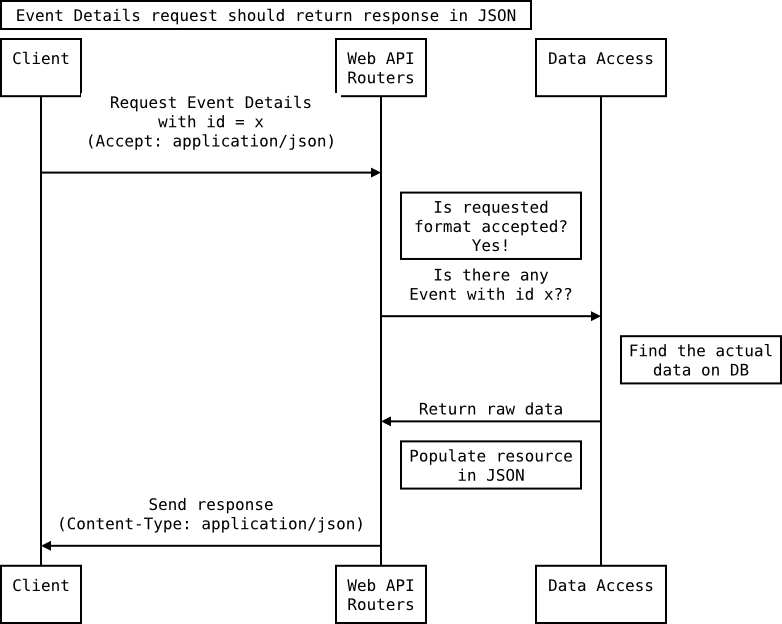
\includegraphics[scale=0.60]{images/event-details-request-seq-diagram-json.png}
\caption{Permintaan Detail Event dalam Format JSON}
\label{event-details-request-seq-diagram-json}
\end{figure}

\newpage

\subsection{Permintaan Detail Event dalam format XML}

\onehalfspacing Pemodelan interaksi antara \textit{client} dan Web API \textit{server} saat \textit{client} meminta detail event dalam format XML dapat dilihat pada gambar \ref{event-details-request-seq-diagram-xml}.

\begin{figure}[htp]
\centering
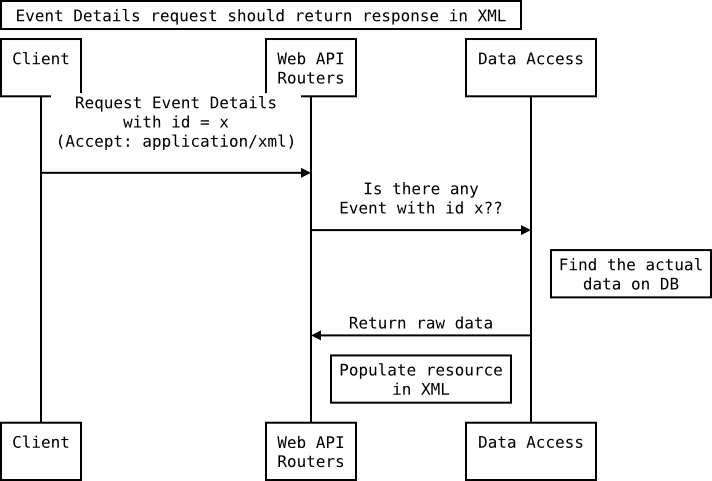
\includegraphics[scale=0.60]{images/event-details-request-seq-diagram-xml.png}
\caption{Permintaan Detail Event dalam Format XML}
\label{event-details-request-seq-diagram-xml}
\end{figure}

\newpage

\subsection{Permintaan Daftar Event dalam format JSON}

\onehalfspacing Pemodelan interaksi antara \textit{client} dan Web API \textit{server} saat \textit{client} meminta daftar event dalam format JSON dapat dilihat pada gambar \ref{event-list-request-seq-diagram-json}.

\begin{figure}[htp]
\centering
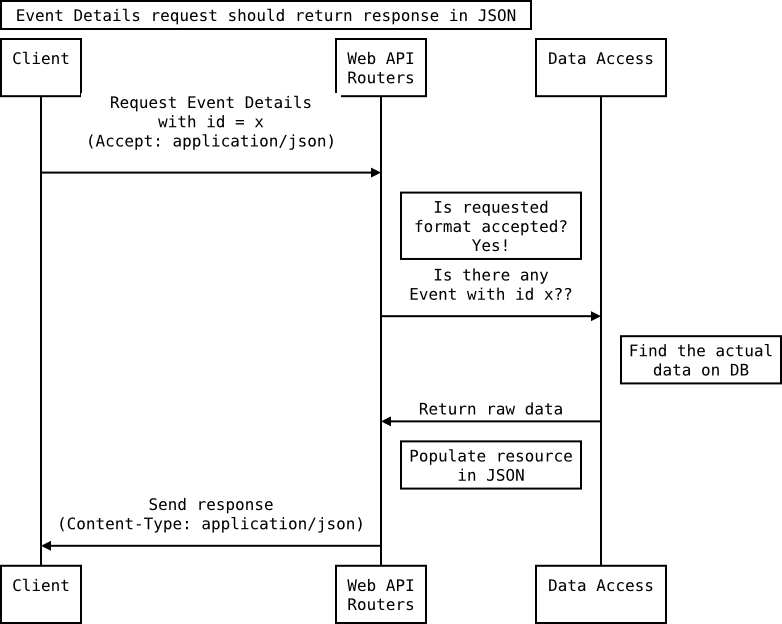
\includegraphics[scale=0.60]{images/event-details-request-seq-diagram-json.png}
\caption{Permintaan Daftar Event dalam Format JSON}
\label{event-list-request-seq-diagram-json}
\end{figure}

\newpage

\subsection{Permintaan Daftar Event dalam format XML}

\onehalfspacing Pemodelan interaksi antara \textit{client} dan Web API \textit{server} saat \textit{client} meminta daftar event dalam format XML dapat dilihat pada gambar \ref{event-list-request-seq-diagram-xml}.

\begin{figure}[htp]
\centering
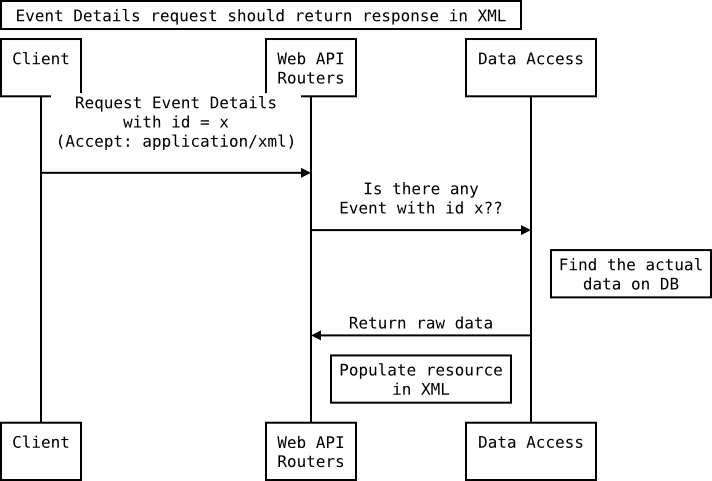
\includegraphics[scale=0.60]{images/event-details-request-seq-diagram-xml.png}
\caption{Permintaan Daftar Event dalam Format XML}
\label{event-list-request-seq-diagram-xml}
\end{figure}

\newpage

\section{Struktur URI}

\onehalfspacing Web API diakses melalui \textit{HTTP endpoints}. \textit{HTTP endpoints} tersebut merupakan struktur URI (\textit{Uniform Resource Identifier}) yang digunakan untuk mengakses \textit{resources}. Representasi visual dalam bentuk \textit{Site Diagram} dari struktur URI tersebut bisa dilihat pada gambar \ref{web-api-uri-structure}

\begin{figure}[htp]
\centering
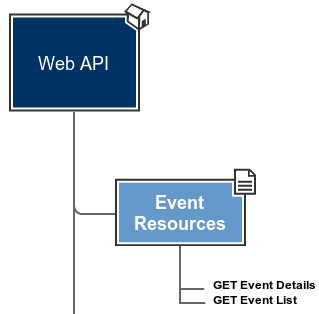
\includegraphics[scale=0.75]{images/web-api-structure.png}
\caption{Struktur URI Web API}
\label{web-api-uri-structure}
\end{figure}

\section{Rancangan Skema Representasi Resource}

\subsection{Pertimbangan Rancangan Skema Representasi Resource dalam format JSON}

\subsubsection{Rancangan Skema Representasi Resource Detail Event dalam format JSON}

\onehalfspacing Berikut adalah beberapa pertimbangan desain untuk rancangan skema representasi \textit{resource} detail event:

\begin{enumerate}
  \item Setiap \textit{resource} detail event akan memiliki URL dalam konteks Web API untuk memberitahukan dimana lokasi \textit{resource} yang diakses
  \item Data aktual detail event akan dibungkus dalam elemen data
\end{enumerate}

Detail rancangan skema dapat dilihat pada lampiran \ref{lampiran:b}.

\subsubsection{Rancangan Skema Representasi Resource Daftar Event dalam format JSON}

\onehalfspacing Berikut adalah beberapa pertimbangan desain untuk rancangan skema representasi \textit{resource} daftar event:

\begin{enumerate}
  \item Setiap \textit{resource} daftar event akan memiliki URL dalam konteks Web API untuk memberitahukan dimana lokasi \textit{resource} yang diakses
  \item Data aktual daftar event akan dibungkus dalam elemen data. Setiap butir event akan dibungkus dalam elemen data yang disertai atribut id.
\item Setiap \textit{resource} daftar event akan disertai properti URL
\end{enumerate}

Detail rancangan skema dapat dilihat pada lampiran \ref{lampiran:b}.

% Daftar buku atau karangan yang merupakan sumber rujukan dari sebuah
% tulisan atau karangan atau daftar tt suatu subjek ilmu, daftar pustaka
% Jumlah maksimal daftar pustaka dan referensi yang bisa dimasukkan adalah 100 item
\begin{thebibliography}{99}
\singlespacing 

% use the surname of the first author, followed by the last two digits of
% the year (hence lamport94)

\bibitem{challenging-issues-and-limitations-of-mobile-computing}
Deepak, G., and Dr. Pradeep B S. "Challenging Issues and Limitations of Mobile Computing."
  \emph{International Journal of Computer Technology and Applications} 3.1 (2012): Academic Journals Database. Web. 8 Jan. 2013.
  
  \bibitem {comparison-of-data-serialization-formats}
Audie Sumaray dan S. Kami Makki. "A comparison of data serialization formats for optimal efficiency on a mobile platform". \emph{6th International Conference on Ubiquitous Information Management and Communication} (2012): Artikel No. 48. ACM Digital Library. Web. 24 Jan 2013.
  
\bibitem{json-vs-xml-debate}
  \emph{Debate: JSON vs. XML as a data interchange format}
  http://www.infoq.com/news/2006/12/json-vs-xml-debate
  diakses pada 20 Januari 2012.
  
\bibitem{serialization-wikipedia}
  \emph{Serialization}
  http://en.wikipedia.org/wiki/Serialization
  diakses pada 24 Januari 2012.
  
\bibitem{agile-wikipedia}
  \emph{Agile software development}
  http://en.wikipedia.org/wiki/Agile\_software\_development
  diakses pada 24 Januari 2012.
  
\bibitem{json-fat-free}
  \emph{JSON: The Fat-Free Alternative to XML}
  http://www.json.org/xml.html
  diakses pada 20 Januari 2012.
  
\bibitem{multitier-architecture-wikipedia}
  \emph{Wikipedia: Multitier architecture}
  http://en.wikipedia.org/wiki/Multitier\_architecture
  diakses pada 15 Maret 2013.
  
\bibitem{three-tier-architecture}
  \emph{Three-Tier Architecture}
  http://www.linuxjournal.com/article/3508
  diakses pada 18 Maret 2013.
  
\bibitem{api-wikipedia}
  \emph{Application Programming Interface}
  http://en.wikipedia.org/wiki/Application\_programming\_interface
  diakses pada 22 Maret 2013.
  
\bibitem{web-api}
  \emph{Web API}
  http://en.wikipedia.org/wiki/Web\_API
  diakses pada 20 Januari 2013.
  
\bibitem{apis-linux-journal}
  \emph{APIs}
  http://www.linuxjournal.com/content/apis
  diakses pada 20 Januari 2013.

\bibitem{ws-restful}
  \emph{RESTful Web services: The basics}
  \\http://www.ibm.com/developerworks/webservices/library/ws-restful/
  diakses pada 14 September 2012.

\bibitem{introducing-json}
  \emph{Introducing JSON} http://www.json.org/
  diakses pada 20 Januari 2013.
  
\bibitem{rfc-4627}
  \emph{The application/json Media Type for JavaScript Object Notation (JSON)} http://tools.ietf.org/html/rfc4627
  diakses pada 5 April 2013.
    
\bibitem{rest-soap}
  \emph{How REST replaced SOAP on the Web: What it means to you}
  http://www.infoq.com/articles/rest-soap
  diakses pada 14 September 2012.
  
\bibitem{xml-wikipedia}
  \emph{XML}
  http://en.wikipedia.org/wiki/XML
  diakses pada 7 April 2013.
  
\bibitem{json-continue-to-winning}
  \emph{JSON Continues its Winning Streak Over XML}
  http://blog.programmableweb.com/2010/12/03/json-continues-its-winning-streak-over-xml/
  diakses pada 8 April 2013.
  
\bibitem{json-continue-to-push}
  \emph{Why JSON will continue to push XML out of the picture}
  http://blog.appfog.com/why-json-will-continue-to-push-xml-out-of-the-picture/
  diakses pada 8 April 2013.
  
\bibitem{acceptance-testing-wikipedia}
  \emph{Acceptance Testing}
  http://en.wikipedia.org/wiki/Acceptance\_testing
  diakses pada 7 Mei 2013.

\bibitem{agile-manifesto}
  \emph{Manifesto Pengembangan Perangkat Lunak Agile}
  http://agilemanifesto.org/iso/id/
  diakses pada 8 April 2013.
  
\bibitem{agile-samurai}
  \emph{The Agile Samuari}
  buku teks
  
\bibitem{introducing-bdd}
  \emph{Introducing BDD}
  http://dannorth.net/introducing-bdd/
  diakses pada 7 Mei 2013.
  
\bibitem{whats-in-story}
  \emph{What's in a Story?}
  http://dannorth.net/whats-in-a-story/
  diakses pada 7 Mei 2013.

\bibitem{jbge-scott}
  \emph{"Just Barely Good Enough" Models and Documents: An Agile Best Practice}
  http://www.agilemodeling.com/essays/barelyGoodEnough.html
  diakses pada 10 Mei 2013.
 
\end{thebibliography}

\appendix
\chapter{Acceptance Criteria} \label{lampiran:a}
\section{Get Event Details Acceptance Criteria}
\subsection{Scenario 1: Event Details request should return response in JSON}

\onehalfspacing \textit{Given Event Details resource is accessible\\
And Event Details resource is accessible\\
When the client request the Event Details in JSON\\
Then the Web API should return Event Details in JSON\\
And returned response is supplied with the Event Details resource URL\\}

\subsection{Scenario 2: Event Details request should return response in XML}

\onehalfspacing \textit{Given Event Details resource is accessible\\
And Event Details resource is accessible\\
When the client request the Event Details in XML\\
Then the Web API should return Event Details in XML\\
And returned response is supplied with the Event Details resource URL\\}

\subsection{Scenario 3: Unsupported Content-Type should return HTTP 406 code}

\onehalfspacing \textit{Given the Web API only support JSON and XML for the response\\
When the client request the resource with Content-Type other than JSON or XML\\
Then the Web API should return HTTP 406 code\\
And returned reponse should be contained an client error message}

\section{Get Event List Acceptance Criteria}

\subsection{Scenario 1: Event List request should return response in JSON}

\onehalfspacing \textit{Given Event List resource is accessible\\
And Event List resource is accessible\\
When the client request the Event List in JSON\\
Then the Web API should return Event List in JSON\\
And returned response is should be accompanied by properties like resource url, page, pages, pageSize, total\\
And the maximum of number of item on the Event List is 15 Event}

\subsection{Scenario 2: Event List request should return response in XML}

\onehalfspacing \textit{Given Event List resource is accessible\\
And Event List resource is accessible\\
When the client request the Event List in XML\\
Then the Web API should return Event List in XML\\
And returned response is should be accompanied by properties like resource url, page, pages, pageSize, total\\
And the maximum of number of item on the Event List is 15 Event}

\subsection{Scenario 3: Unsupported Content-Type should return HTTP 406 code}

\onehalfspacing \textit{Given the Web API only support JSON and XML for the response\\
When the client request the resource with Content-Type other than JSON or XML\\
Then the Web API should return HTTP 406 code\\
And returned reponse should be contained an client error message}

\chapter{Detail Rancangan Skema Representasi Resource} \label{lampiran:b}
\section{Rancangan Skema Representasi Resource Detail Event}
\subsection{Rancangan Skema Representasi Resource Detail Event dalam format JSON}
\onehalfspacing Tanpa menghiraukan nilai dari masing-masing \textit{field}, berikut adalah rancangan skema representasi \textit{resource} detail event dalam format JSON:

\begin{lstlisting}[frame=single]
{
  "url": value,
  "data":  {
    "title": value,
      "shortDescription": value,
      "times": [
        {
          "milliseconds": value,
          "fullFormat": value,
          "year": value,
          "month": value,
          "date": value,
          "day": value
        }
      ],
      "isPassed": value,
      "rating": value,
      "lastUpdated": value,
      "timestamp": value,
      "_id": "value"
    }
}
\end{lstlisting}

\onehalfspacing Untuk melihat detail dari setiap contoh nilai setiap \textit{field} dari rancangan skema di atas, silahkan untuk melihatnya di halaman web \textit{ghanoz-json: Event Details resource representations design in JSON}\footnote{https://gist.github.com/muhammadghazali/5409322\#file-event-details-json}

\subsection{Rancangan Skema Representasi Resource Detail Event dalam format XML}
\onehalfspacing Tanpa menghiraukan nilai dari masing-masing \textit{field}, berikut adalah rancangan skema representasi \textit{resource} detail event dalam format XML:

\begin{lstlisting}[frame=single]
<response>
    <url>value</url>
    <data id="1">
        <title>value</title>
        <shortDescription>value</shortDescription>
        <times>
            <time>
                <milliseconds>value</milliseconds>
                <fullFormat>value</fullFormat>
                <year>value</year>
                <month>value</month>
                <date>value</date>
                <day>value</day>
            </time>
        </times>
        <isPassed>value</isPassed>
        <rating>value</rating>
        <lastUpdated>value</lastUpdated>
        <timestamp>value</timestamp>
    </data>
</response>
\end{lstlisting}

\onehalfspacing Untuk melihat detail dari setiap contoh nilai setiap \textit{field} dari rancangan skema di atas, silahkan untuk melihatnya di halaman web \textit{ghanoz-json: Event Details resource representations design in XML}\footnote{https://gist.github.com/muhammadghazali/5409508\#file-event-details-xml}

\section{Rancangan Skema Representasi Resource Daftar Event}

\onehalfspacing Tanpa menghiraukan nilai dari masing-masing \textit{field}, berikut adalah rancangan skema representasi \textit{resource} detail event dalam format JSON:

\begin{lstlisting}[frame=single]
{
  "url": value,
  "data": [
    {
      "title": value,
      "shortDescription": value,
      "times": [
        {
          "milliseconds": value,
          "fullFormat": value,
          "year": value,
          "month": value,
          "date": value,
          "day": value
        }
      ],
      "isPassed": value,
      "rating": value,
      "lastUpdated": value,
      "timestamp": value,
      "_id": value
    },
    {
      "title": value,
      "shortDescription": value,
      "times": [
        {
          "milliseconds": value,
          "fullFormat": value,
          "year": value,
          "month": value,
          "date": value,
          "day": value
        }
      ],
      "isPassed": value,
      "rating": value,
      "lastUpdated": value,
      "timestamp": value,
      "_id": value
    }
  ]
}
\end{lstlisting}

\onehalfspacing Untuk melihat detail dari setiap contoh nilai setiap \textit{field} dari rancangan skema di atas, silahkan untuk melihatnya di halaman web \textit{ghanoz-json: Event List resource representations design in JSON}\footnote{https://gist.github.com/muhammadghazali/5409417\#file-event-list-json}

\subsection{Rancangan Skema Representasi Resource Daftar Event dalam format XML}
\onehalfspacing Tanpa menghiraukan nilai dari masing-masing \textit{field}, berikut adalah rancangan skema representasi \textit{resource} detail event dalam format XML:

\begin{lstlisting}[frame=single]
<response>
    <url>value</url>
    <data>
        <data id="value">
            <title>value</title>
            <shortDescription>value</shortDescription>
            <times>
                <time>
                    <milliseconds>value</milliseconds>
                    <fullFormat>value</fullFormat>
                    <year>value</year>
                    <month>value</month>
                    <date>value</date>
                    <day>value</day>
                </time>
            </times>
            <isPassed>value</isPassed>
            <rating>value</rating>
            <lastUpdated>value</lastUpdated>
            <timestamp>value</timestamp>
        </data>
        <data id="value">
            <title>value</title>
            <shortDescription>value</shortDescription>
            <times>
                <time>
                    <milliseconds>value</milliseconds>
                    <fullFormat>value</fullFormat>
                    <year>value</year>
                    <month>value</month>
                    <date>value</date>
                    <day>value</day>
                </time>
            </times>
            <isPassed>value</isPassed>
            <rating>value</rating>
            <lastUpdated>value</lastUpdated>
            <timestamp>value</timestamp>
        </data>
    </data>
</response>
\end{lstlisting}

\onehalfspacing Untuk melihat detail dari setiap contoh nilai setiap \textit{field} dari rancangan skema di atas, silahkan untuk melihatnya di halaman web \textit{ghanoz-json: Event Details resource representations design in XML}\footnote{https://gist.github.com/muhammadghazali/5409528\#file-event-list-xml}

\end{document}